\documentclass{article}

\usepackage{fullpage}
\usepackage{graphicx}
\usepackage{color}
\usepackage{fancyhdr}
\usepackage{url}
\usepackage{subfig}
\usepackage{amsmath,bm}
\usepackage{amssymb}
\usepackage{amsthm}
\usepackage{amsfonts}
\usepackage[round]{natbib}
\usepackage{enumitem,xcolor}
\usepackage[multiple]{footmisc}

\usepackage[
 pdftitle={Capstone Report - Udacity Machine Learning Nanodegree},
 pdfsubject={Machine Learning, Reinforcement Learning, Deep Learning, Artificial Intelligence, Games},
 pdfauthor={David Robles},
 pdfpagemode=UseOutlines,
 pdfborder= {0 0 1.0},
 bookmarks,
 bookmarksopen,
 colorlinks=true,
 citecolor=blue,
 linkcolor=blue, %
 linkbordercolor=blue, %
 urlcolor=blue, %
]{hyperref}

\usepackage[labelfont=bf]{caption}


\usepackage[utf8]{inputenc}

% Default fixed font does not support bold face
\DeclareFixedFont{\ttb}{T1}{txtt}{bx}{n}{8} % for bold
\DeclareFixedFont{\ttm}{T1}{txtt}{m}{n}{8}  % for normal

% Custom colors
\usepackage{color}
\definecolor{deepblue}{rgb}{0,0,0.5}
\definecolor{deepred}{rgb}{0.6,0,0}
\definecolor{deepgreen}{rgb}{0,0.5,0}

\usepackage{listings}

\definecolor{codebg}{RGB}{238,238,238}

% Python style for highlighting
\newcommand\pythonstyle{\lstset{
language=Python,
basicstyle=\ttm,
otherkeywords={self},             % Add keywords here
keywordstyle=\ttb\color{deepblue},
emph={MyClass,__init__},          % Custom highlighting
emphstyle=\ttb\color{deepred},    % Custom highlighting style
stringstyle=\color{deepgreen},
frame=tb,                         % Any extra options here
framesep=10pt,
framexleftmargin=10pt,
backgroundcolor=\color{codebg},
rulecolor=\color{codebg},
aboveskip=15pt,
belowskip=15pt,
showstringspaces=false            % 
}}


% Python environment
\lstnewenvironment{python}[1][]
{
\pythonstyle
\lstset{#1}
}
{}

% Python for external files
\newcommand\pythonexternal[2][]{{
\pythonstyle
\lstinputlisting[#1]{#2}}}

% Python for inline
\newcommand\pythoninline[1]{{\pythonstyle\lstinline!#1!}}

%%%%%%%%%%%%%%%%%%%%%%%%%%%%%%%%%%%%%%%%%%%%%%%%%%%%%%%%%%%%%%%%%%%%%%%%%%%%%%%%%%%%%%%%%%%%%%%%%%%%
\title{Machine Learning Nanodegree \\ Capstone Report}
\author{David A. Robles}
\date{January 31, 2017}
\begin{document}
\maketitle
%%%%%%%%%%%%%%%%%%%%%%%%%%%%%%%%%%%%%%%%%%%%%%%%%%%%%%%%%%%%%%%%%%%%%%%%%%%%%%%%%%%%%%%%%%%%%%%%%%%%

%%%%%%%%%%%%%%%%%%%%%%%%%%%%%%%%%%%%%%%%%%%%%%%%%%%%%%%%%%%%%%%%%%%%%%%%%%%%%%%%%%%%%%%%%%%%%%%%%%%%
\section{Definition}
%%%%%%%%%%%%%%%%%%%%%%%%%%%%%%%%%%%%%%%%%%%%%%%%%%%%%%%%%%%%%%%%%%%%%%%%%%%%%%%%%%%%%%%%%%%%%%%%%%%%

%%%%%%%%%%%%%%%%%%%%%%%%%%%%%
\subsection{Project Overview}
%%%%%%%%%%%%%%%%%%%%%%%%%%%%%

Content.

%%%%%%%%%%%%%%%%%%%%%%%%%%%%%%
\subsection{Problem Statement}
\label{sec:problem-statement}
%%%%%%%%%%%%%%%%%%%%%%%%%%%%%%

\newcommand{\URLcf}{https://en.wikipedia.org/wiki/Connect_Four}

In this project, we will use reinforcement learning with deep learning to make an agent learn to
play the game of {Connect 4}\footnote{\url{\URLcf}} by playing games against itself. In other words,
using the formalism used by \cite{Mitchell1997Book} to define a machine learning problem:

\begin{itemize}

    \item \textbf{Task:} Playing Connect 4.

    \item \textbf{Performance:} Percent of games won against other agents, and accuracy of the
        predictions on a Connect 4 dataset.

    \item \textbf{Experience:} Games played against itself.

    \item \textbf{Target function:} $Q^\pi : \mathcal{S} \times \mathcal{A} \to \mathbb{R}$, where
        $\mathcal{S}$ is the set of \emph{states} (board positions) and $\mathcal{A}$ is the set of
        \emph{actions} (moves), and $\mathbb{R}$ represents the value of being in a state $s \in
        \mathcal{S}$, applying a action $a \in \mathcal{A}$, and following policy $\pi$ thereafter.

    \item \textbf{Target function representation:} Deep neural network.

\end{itemize}

Therefore, I seek to build a Q-learning agent trained via a deep convolutional neural network to
approximate the optimal action-value function:

\begin{equation}
Q^*(s,a) = \max\limits_\pi Q^\pi(s,a), \forall s \in \mathcal{S}, a \in \mathcal{A}
\end{equation}

\noindent which is the maximum sum of rewards achievable by a behaviour policy $\pi$.

%%%%%%%%%%%%%%%%%%%%
\subsection{Metrics}
%%%%%%%%%%%%%%%%%%%%

\begin{itemize}

    \item \textbf{Winning percentage.} This metric consists in playing a high number of games (e.g.
        100,000) against another agent (e.g. a random agent), and calculating the average of games
        won by the agent that uses the learned value function.
        
    \item \textbf{Prediction accuracy.} The learned value function will be used to predict the
        game-theoretic outcomes (win, loss or draw) of the board positions in the Connect 4 Data
        Set.

\end{itemize}

%%%%%%%%%%%%%%%%%%%%%%%%%%%%%%%%%%%%%%%%%%%%%%%%%%%%%%%%%%%%%%%%%%%%%%%%%%%%%%%%%%%%%%%%%%%%%%%%%%%%
\section{Analysis}
%%%%%%%%%%%%%%%%%%%%%%%%%%%%%%%%%%%%%%%%%%%%%%%%%%%%%%%%%%%%%%%%%%%%%%%%%%%%%%%%%%%%%%%%%%%%%%%%%%%%

%%%%%%%%%%%%%%%%%%%%%%%%%%%%%
\subsection{Data Exploration}
%%%%%%%%%%%%%%%%%%%%%%%%%%%%%

Content.

%%%%%%%%%%%%%%%%%%%%%%%%%%%%%%%%%%%%%%
\subsection{Exploratory Visualization}
%%%%%%%%%%%%%%%%%%%%%%%%%%%%%%%%%%%%%%

Content.

%%%%%%%%%%%%%%%%%%%%%%%%%%%%%%%%%%%%%%
\subsection{Algorithms and Techniques}
%%%%%%%%%%%%%%%%%%%%%%%%%%%%%%%%%%%%%%

%%%%%%%%%%%%%%%%%%%%%%%%%%%%%%%%%%
\subsubsection{Alpha-beta pruning}
%%%%%%%%%%%%%%%%%%%%%%%%%%%%%%%%%%

\noindent
\href{https://github.com/davidrobles/mlnd-capstone-code/blob/master/capstone/player/alphabeta.py}
     {Implementation}
\break

% In this project, we will use reinforcement learning with deep learning to make an agent learn to
% play the game of {Connect 4}\footnote{\url{\URLcf}} by playing games against itself. In other words,
% using the formalism used by \cite{Mitchell1997Book} to define a machine learning problem:

\emph{Alpha-beta pruning}~\citep{Knuth1975AB} is the most common game tree search algorithm for
two-player games of perfect information. It extends the minimax algorithm to reduce the number of
nodes that are evaluated in the game tree. Instead of calculating the exact minimax values for all
the nodes in the game tree, alpha-beta prunes away branches that will not have any effect in the
selection of the best move.

% \hyperref[fig:ab-game-tree]{Figure~\ref*{fig:ab-game-tree}} illustrates
% the prunning process in the Alpha-Beta algorithm. This tree has a total of 28 nodes, however, 10
% nodes of the tree were pruned (crossed branches) because those branches do not have any effect in
% the selection of the best move.

% The algorithm works by imposing a \emph{search window} $\left[ \alpha, \beta \right] $ at each
% \textsc{Min} or \textsc{Max} node in the game tree. $\alpha$ represents the value of the best (i.e.
% highest-value) node found so far for \textsc{Max}, while $\beta$ is the best value (i.e.
% lowest-value) for \textsc{Min}. The search through successor nodes can be terminated as soon as the
% current node's value is proven to fall outside the search window. The functionality of Alpha-Beta
% is detailed in \hyperref[alg:alpha-beta]{Algorithm~\ref*{alg:alpha-beta}}.

% \newcommand{\URLab}{https://github.com/davidrobles/mlnd-capstone-code/blob/master/capstone/player/alphabeta.py}

%%%%%%%%%%%%%%%%%%%%%%%%%%
\subsubsection{Q-learning}
%%%%%%%%%%%%%%%%%%%%%%%%%%

\noindent \href{https://github.com/davidrobles/mlnd-capstone-code/blob/master/capstone/algorithms/qlearning.py}
     {Implementation}
\break

One of the most basic and popular methods to estimate action-value functions is the
\emph{Q-learning} algorithm~\citep{Watkins1989PhD}. It is model-free online off-policy algorithm,
whose main strength is that it is able to compare the expected utility of the available actions
without requiring a model of the environment. Q-learning works by learning an action-value function
that gives the expected utility of taking a given action in a given state and following a fixed
policy thereafter. The update rule uses action-values and a built-in max-operator over the
action-values of the next state in order to update $Q(s_t, a_t)$ as follows,
%
\begin{equation}
    Q(s_t, a_t) \gets Q(s_t, a_t) + \alpha [r_{t+1} + \gamma \max_a Q(s_{t+1}, a) - Q(s_t, a_t)]
\end{equation}

The agent makes a step in the environment from state $s_t$ to $s_{t+1}$ using action $a_t$ while
receiving reward $r_t$. The update takes place on the action-value $a_t$ in the state $s_t$ from
which this action was executed.

Q-learning is exploration-intensive, which means that it will converge to the optimal policy
regardless of the exploration policy being followed, under the assumption that each state-action
pair is visited an infinite number of times, and the learning parameter $\alpha$ is decreased
appropriately~\citep{Watkins1992Q}.

\subsubsection{Self-play}

Self-play is by far the most popular training method. It is a single policy $\pi(s,a)$ that is used
by both players in a two-player game, $\pi_1(s,a) = \pi_2(s,a) = \pi(s,a)$. The first reason for its
popularity is that training is quickest if the learner's opponent is roughly equally strong, and
that definitely holds for self-play. As a second reason for popularity, there is no need to
implement or access a different agent with roughly equal playing strength. However, self-play has
several drawbacks, with the main one being that a single opponent does not provide sufficient
exploration~\citep{Szita2011RLGames}.

%%%%%%%%%%%%%%%%%%%%%%
\subsection{Benchmark}
\label{sec:benchmark}
%%%%%%%%%%%%%%%%%%%%%%

\begin{itemize}

    \item \textbf{Random agent}. This benchmark consists in playing against an agent that takes
        uniformly random moves. This is the most basic benchmark, but first we have to be sure that
        our learned evaluation function can play better than a random agent before moving into a
        harder benchmark. Also, this will help us to detect bugs in the code and algorithms: if a
        learned value function does not play significantly better than a random agent, is not
        learning. The idea is to test against this benchmark using Alpha-beta pruning at 1, 2 and
        4-ply search.

    \item \textbf{Connect 4 Data Set}. This dataset will be used as the main benchmark. The learned
        value function will be used to predict the game-theoretic outcomes (win, loss or draw) for
        the first player in the 67,557 instances of the dataset.

\end{itemize}

%%%%%%%%%%%%%%%%%%%%%%%%%%%%%%%%%%%%%%%%%%%%%%%%%%%%%%%%%%%%%%%%%%%%%%%%%%%%%%%%%%%%%%%%%%%%%%%%%%%%
\section{Implementation}
%%%%%%%%%%%%%%%%%%%%%%%%%%%%%%%%%%%%%%%%%%%%%%%%%%%%%%%%%%%%%%%%%%%%%%%%%%%%%%%%%%%%%%%%%%%%%%%%%%%%

%%%%%%%%%%%%%%%%%%%%%%%%%%%%%%%%%%%%
\subsection{Markov Decision Process}
%%%%%%%%%%%%%%%%%%%%%%%%%%%%%%%%%%%%

\noindent
\href{https://github.com/davidrobles/mlnd-capstone-code/blob/master/capstone/mdp/mdp.py}
     {Implementation}
\break

A \emph{Markov decision process} (MDP) consist of a set of states, a set of actions, a transition
function and a reward function.

\begin{itemize}

    \item $\mathcal{S}$ is the set of \emph{states} (state space).

    \item $\mathcal{A}$ is the set of \emph{actions} (action space). The set of actions that are
      available in some particular state $s_t \in \mathcal{S}$ is denoted $\mathcal{A}(s_t)$, such
      that $\mathcal{A}(s_t) \in \mathcal{P}(\mathcal{A})$, where $\mathcal{P}(\cdot)$ denotes the
      power set.

    \item $ T : \mathcal{S} \times \mathcal{A} \times \mathcal{S} \to \mathbb{R}$ is the
      \emph{transition function}, which is the probability given we are in state $s_t \in
      \mathcal{S}$, take action $a_t \in \mathcal{A}(s_t)$ and we will transition to state $s_{t+1}
      \in \mathcal{S}$.

    \item $ R : \mathcal{S} \times \mathcal{A} \times \mathcal{S} \to \mathbb{R}$ is the
      \emph{reward function}, which is the immediate reward received when in state $s_t \in
      \mathcal{S}$ action $a_t \in \mathcal{A}$ is taken and the MDP transitions to state $s_{t+1}
      \in \mathcal{S}$. However, it is also possible to define it either as $ R : \mathcal{S} \times
      \mathcal{A} \to \mathbb{R}$ or $R : \mathcal{S} \to \mathbb{R}$. The first one gives rewards
      for performing an action $a_t$ in a particular state $s_t$, and the second gives rewards when
      transitioning to state $s_{t+1}$.

\end{itemize}

%%%%%%%%%%%%%%%%%%%%%%%%
\subsection{Environment}
%%%%%%%%%%%%%%%%%%%%%%%%

\noindent
\href{https://github.com/davidrobles/mlnd-capstone-code/blob/master/capstone/environment/environment.py}
     {Implementation}
\break

An agent does not have access to the dynamics (reward and transition function) of the MDP. However,
it interacts with an \emph{environment} by way of three signals: a \emph{state}, which describes the
state of the environment, an \emph{action}, which allows the agent to have some impact on the
environment, and a \emph{reward}, which provides the agent with feedback on its immediate
performance.

%%%%%%%%%%%%%%%%%%%
\subsection{Policy}
%%%%%%%%%%%%%%%%%%%

\noindent
\href{https://github.com/davidrobles/mlnd-capstone-code/blob/master/capstone/policy/policy.py}
     {Implementation}
\break

In an MDP, the agent acts according to a policy $\pi$, which maps each state $s \in \mathcal{S}$ to
an action $a \in \mathcal{A}(s)$. A policy that specifies a unique action to be performed is called
a \emph{deterministic} policy, and is defined as $\pi : \mathcal{S} \rightarrow \mathcal{A}$. On the
other hand, a \emph{stochastic} policy $\pi : \mathcal{S} \times \mathcal{A} \rightarrow [0,1]$
selects actions according to a probability distribution, such that for each state $s \in
\mathcal{S}$, it holds that $\pi(s,a) \geq 0$ and $\sum_{a\in\mathcal{A}(s)} \pi(s,a) = 1$.

The interaction between the policy used by the agent and the environment works as follows. First, it
starts at an \emph{initial state} $s_0$. Then, the policy $\pi$ selects an action $a_0 = \pi(s_0)$
from the set of available actions $\mathcal{A}(s_0)$, and the action is executed. The environment
transitions to a new state $s_1$ based on the transition function $T$ with probability
$T(s_0,a_0,s_1)$, and a reward $r_0 = R(s_0, a_0, s_1)$ is received. This process continues,
producing a \emph{trajectory} of experience $s_0, a_0, s_1, r_1, a_1, s_2, r_2, a_2, \dots$. If the
task is \emph{episodic}, the process ends in a \emph{terminal state} $s_T$ and is restarted in the
initial state. If the task is \emph{continiuing}, the sequence of states can be extended
indefinitely.

%%%%%%%%%%%%%%%%%%%%%%%%%%%%%%%%%%%%%%%%%%%%%%%%%%%%%%%%%%%%%%%%%%%%%%%%%%%%%%%%%%%%%%%%%%%%%%%%%%%%
\section{Methodology}
%%%%%%%%%%%%%%%%%%%%%%%%%%%%%%%%%%%%%%%%%%%%%%%%%%%%%%%%%%%%%%%%%%%%%%%%%%%%%%%%%%%%%%%%%%%%%%%%%%%%

%%%%%%%%%%%%%%%%%%%%%%%%%%%%%%%
\subsection{Data Preprocessing}
%%%%%%%%%%%%%%%%%%%%%%%%%%%%%%%

Content.

%%%%%%%%%%%%%%%%%%%%%%%%%%%
\subsection{Implementation}
%%%%%%%%%%%%%%%%%%%%%%%%%%%

\begin{itemize}

    \item Two games were implemented: Tic Tac Toe and Connect 4.
    \item Converting a to an MDP by using a fixed agent.
    \item Show that q-learning learns to play against a fixed opponent using Tic-Tac-Toe.
    \item Show that q-learning learns to play against a fixed opponent using Connect 4.

\end{itemize}

%%%%%%%%%%%%%%%%%%%%%%%
\subsection{Refinement}
%%%%%%%%%%%%%%%%%%%%%%%

Content.

%%%%%%%%%%%%%%%%%%
\subsection{Games}
%%%%%%%%%%%%%%%%%%

%%%%%%%%%%%%%%%%%%%%%%%%%%%
\subsubsection{Tic Tac Toe}
%%%%%%%%%%%%%%%%%%%%%%%%%%%

\noindent
\href{https://github.com/davidrobles/mlnd-capstone-code/blob/master/capstone/game/tictactoe.py}
     {Implementation}
\break

%%%%%%%%%%%%%%%%%%%%%%%%%
\subsubsection{Connect 4}
%%%%%%%%%%%%%%%%%%%%%%%%%

\noindent
\href{https://github.com/davidrobles/mlnd-capstone-code/blob/master/capstone/game/connect4.py}
     {Implementation}
\break

Connect 4 is a two-player board game of perfect information where pieces are dropped into the
columns of a vertical $6 \times 7$ grid with the goal of forming a straight line of 4 connected
pieces. There are at most 7 actions per state, since placing a piece in a column is a legal action
only if that column has at least one empty location. \hyperref[fig:c4-game]{Figure~\ref*{fig:c4-game}}
shows three Connect 4 game positions. 

%%%%%%%%%%
% Figure %
%%%%%%%%%%

\begin{figure}[!h]
    \centering
    \subfloat[Win for \textsc{Player 1}]{
        \label{fig:c4-game-1}
        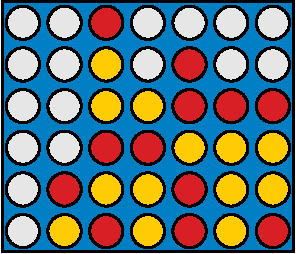
\includegraphics[width=0.3\textwidth]{figures/c4/c4-win-blue-c5f2.pdf}
    } \hspace{0.1in}
    \subfloat[Win for \textsc{Player 2}]{
        \label{fig:c4-game-2}
        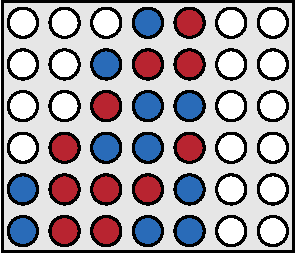
\includegraphics[width=0.3\textwidth]{figures/c4/c4-win-red-b3e6.pdf}
    } \hspace{0.1in}
    \subfloat[Draw]{
        \label{fig:c4-game-3}
        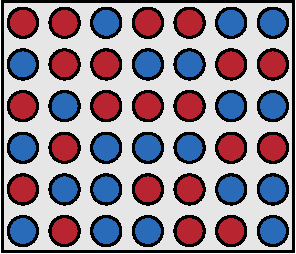
\includegraphics[width=0.3\textwidth]{figures/c4/c4-draw.pdf}
    }
    \caption{Examples of wins, losses and draws in Connect Four}
    \label{fig:c4-game}
\end{figure}


\subsubsection{GameMDP converter}

Converting an MDP

%%%%%%%%%%%%%%%%%%%%%%%%%%%%%%%%%%%%%%%%%%%%%%%%%%%%%%%%%%%%%%%%%%%%%%
\subsubsection{Learn Tic-Tac-Toe state-action values using Q-learning}
%%%%%%%%%%%%%%%%%%%%%%%%%%%%%%%%%%%%%%%%%%%%%%%%%%%%%%%%%%%%%%%%%%%%%%

% - Implement Q-learning
% - GameMDP converter
% - Generate a Tic-Tac-Toe board that is easier to analyze
% - Run Q-learning and show that the values are correct.

\noindent
\href{https://github.com/davidrobles/mlnd-capstone-code/blob/master/examples/tictactoe-qlearning.py}
     {Implementation}
\break

First, we will test our q-learning algorithm by learning the state action values for an agent that
plays against a fixed tic tac toe player. this fixed tic tac toe player will be an AlphaBeta player,
which means it will always make an optimal move. An optimal move means that is the best possible
move in that situation.

We created a custom board position that is small but that it can demonstrate the idea of learning
the q-learning values.

The situation consists where we are in the following position:

%%%%%%%%%%
% Figure %
%%%%%%%%%%

\begin{figure}[!h]
    \centering
    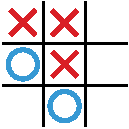
\includegraphics[width=0.15\textwidth]{figures/tic/tic-1.pdf}
    \caption{Tic-Tac-Toe board, $s$, with five legal moves: $\{2, 3, 6, 7, 9\}$.}
    \label{fig:tic-play32}
\end{figure}

In this position the player X is next, and it has 5 available moves: 1, 3, 6, 9.

% show the index nubmers of the board

We ran the Q-learning algorithm with the following parameters and these are the results:

% add link to script here.

%%%%%%%%%%
% Figure %
%%%%%%%%%%

\begin{figure}[!h]
    \centering
    \subfloat[$Q(s, 2) = 0.9895$]{
        \label{fig:tic-game-1}
        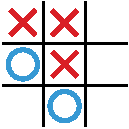
\includegraphics[width=0.15\textwidth]{figures/tic/tic-1.pdf}
    } \hspace{0.1in}
    \subfloat[$Q(s, 3) = 0.9897$]{
        \label{fig:tic-game-2}
        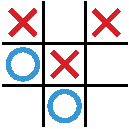
\includegraphics[width=0.15\textwidth]{figures/tic/tic-2.pdf}
    } \hspace{0.1in}
    \subfloat[$Q(s, 6) = 0.0$]{
        \label{fig:tic-game-3}
        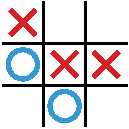
\includegraphics[width=0.15\textwidth]{figures/tic/tic-3.pdf}
    } \hspace{0.1in}
    \subfloat[$Q(s, 7) = 0.9890$]{
        \label{fig:tic-game-4}
        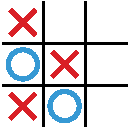
\includegraphics[width=0.15\textwidth]{figures/tic/tic-4.pdf}
    } \hspace{0.1in}
    \subfloat[$Q(s, 9) = 0.9999$]{
        \label{fig:tic-game-4}
        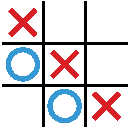
\includegraphics[width=0.15\textwidth]{figures/tic/tic-5.pdf}
    }
    \caption{}
    \label{fig:tic-play}
\end{figure}

As we can see we were able to learn the state-action values for each board position. It
is clear that the best board is the one that leads to a direct win, and the other boards
lead to either draws (like in...) or a loss.

Now we will run the same algorithm but starting from the initial position. 

% add link, and add random_state to algorithms

As we can see it learned to play perfectly against an alpha-beta player.

With this example we can confirm that the implementation of our q-learning algorithm
is working fine, and now we can move into our next step.

%%%%%%%%%%%%%%%%%%%%%%%%%%%%%%%%%%%%%%%%%%%%%%%%%%%%%%%%%%%%%%%%%%%%%%%%%%%%%%%%%%%%%%%%%%%%%%%%%%%%
\section{Results}
%%%%%%%%%%%%%%%%%%%%%%%%%%%%%%%%%%%%%%%%%%%%%%%%%%%%%%%%%%%%%%%%%%%%%%%%%%%%%%%%%%%%%%%%%%%%%%%%%%%%

%%%%%%%%%%%%%%%%%%%%%%%%%%%%%%%%%%%%%%%%%%%%
\subsection{Model Evaluation and Validation}
%%%%%%%%%%%%%%%%%%%%%%%%%%%%%%%%%%%%%%%%%%%%

Content.

%%%%%%%%%%%%%%%%%%%%%%%%%%
\subsection{Justification}
%%%%%%%%%%%%%%%%%%%%%%%%%%

Content.

%%%%%%%%%%%%%%%%%%%%%%%%%%%%%%%%%%%%%%%%%%%%%%%%%%%%%%%%%%%%%%%%%%%%%%%%%%%%%%%%%%%%%%%%%%%%%%%%%%%%
\section{Conclusion}
%%%%%%%%%%%%%%%%%%%%%%%%%%%%%%%%%%%%%%%%%%%%%%%%%%%%%%%%%%%%%%%%%%%%%%%%%%%%%%%%%%%%%%%%%%%%%%%%%%%%

%%%%%%%%%%%%%%%%%%%%%%%%%%%%%%%%%%%%
\subsection{Free-Form Visualization}
%%%%%%%%%%%%%%%%%%%%%%%%%%%%%%%%%%%%

Content.

%%%%%%%%%%%%%%%%%%%%%%%
\subsection{Reflection}
%%%%%%%%%%%%%%%%%%%%%%%

Content.

%%%%%%%%%%%%%%%%%%%%%%%%
\subsection{Improvement}
%%%%%%%%%%%%%%%%%%%%%%%%

Content.

%%%%%%%%%%%%%%%%%%%%%%%%%%%%%%%%%%%%%%%%%%%%%%%%%%%%%%%%%%%%%%%%%%%%%%%%%%%%%%%%%%%%%%%%%%%%%%%%%%%%
% BIBLIOGRAPHY
%%%%%%%%%%%%%%%%%%%%%%%%%%%%%%%%%%%%%%%%%%%%%%%%%%%%%%%%%%%%%%%%%%%%%%%%%%%%%%%%%%%%%%%%%%%%%%%%%%%%

\bibliographystyle{plainnat}
\bibliography{bibliography}

\end{document}
